\documentclass[a4paper]{scrartcl}

\usepackage[english]{babel}
\usepackage[utf8]{inputenc}
\usepackage{times}
\usepackage{graphicx}
\usepackage{url}
\usepackage[colorinlistoftodos]{todonotes}
\usepackage{multicol}
\usepackage{wrapfig}

% Look for images in ./images folder.
\graphicspath{{./images/}}

% Front page main information.
\title{\gamename}
\subtitle{Game Design Document}
\author{}
\date{\today}

\begin{document}

% Define the name of the game.
\newcommand{\gamename}{\emph{Ice Cream Factory}}

\maketitle

	\begin{quotation}
		\noindent
		\textit{The production of ice cream is a sweet business. There are so many flavors, so many toppings, so many combinations! The weather is hot and customers are avid for different types of ice cream. So hands-on and starting producing!}
	\end{quotation}

\section{Introduction}
	\gamename is a puzzle game for Windows, Linux, Web, Android and iOS in which the player needs to build an ice cream factory by correct placing cup dispensers, flavor and topping dosers, patch switchers and other devices on a predefined layout of conveyors, in order to produce the different types of ice creams in the requested quantities by customers.
	
	Once the production line is set-up by, the player can start the factory and watch the production happening. A truck driver character supports the fantasy and the mechanics by providing the player with the customer requests (posting orders in simple speech bubbles) and awaiting for the products, giving visual and auditory feedback on the success or failure of the puzzle.
	
	When the factory is running, empty cups are put in the conveyor belt by the cup dispenser and are carried by the conveyors in their indicated roll direction. When the cups get under other equipment they are manipulated by the intended action: for example, when under a flavor doser a scoop of ice cream is dispensed. Therefore, the player needs to put the devices on the conveyor belt \textit{in the correct order} so a specific type of ice cream is gradually composed. For instance, a chocolate with nuts ice cream can be produced by first conducting the empty cup under the chocolate flavor doser and then under the nuts topping doser, finally delivering it to the end of the conveyor belt to the truck driver.
	
	The puzzle difficulty increases with each level. Customers may require ice creams with more than one scoop or with extra toppings, which will require conducting the cups under a given device more than once. Also, the order posted by the truck driver may require different numbers of ice cream types (1 nuts-chocolate and 2 plain-chocolate, for instance). Additionally, the conveyors will form increasingly more complex shapes, requiring careful planing and experimentation for positioning the available equipment to properly satisfy the customer requests.

    The game targets both male and female players with at least 10 years old, without an upper limit of age.
    
    \subsection{Vision Statement}
    	The player should be delivered with the following experiences:
    	\begin{itemize}
    		\item Satisfaction in solving challenging but lighthearted puzzles
    		\item Amusement with the game visual art, music and sound effects
    		\item Curiosity about the behavior of characters and the operation of devices
    	\end{itemize}

	\subsection{Objective}
		In each level the player has to set-up the available devices on the fixed conveyor belt layout in order to produce the amount of ice cream, in their different combinations, as requested by the truck driver.
		
	\subsection{Aesthetics}
		The game has a cartoony style both in its visual and auditory elements, with a 2D isometric projection. The graphical art is simple, colorful and beautiful and the sound effects and music are surprising, bouncy and funny. So, a complete production line feels and sounds like a ``crazy factory'' (while working, the factory will sound like vintage machinery\footnote{\url{http://www.soundsnap.com/node/36489}}).
		
	\subsection{Features}
	    \begin{itemize}
	        \item 3 base ice creams, 4 flavors, 5 toppings, 4 special toppings
	        \item 13 different devices
	        \item Over 100 levels
	        \item Mind blowing puzzles
	    \end{itemize}
	
	\subsection{Target platforms}
	    \gamename is a simple and casual game, making it ideal for browser, tablets
	    and PC. Players will interact with the game by touch (in case of tablets) or with the mouse cursor (in case of browser and PC). The targeted platforms are Android, iOS, Windows and Linux.
		
\section{Game Elements}

	\subsection{Characters}

		\subsubsection{The Player}
			The player has no avatar in the game, being intrinsically known as the owner of the ice cream factory. When interacting with the player, other characters will look towards the screen, for that matter. The player interacts with the game by touching the screen in version for mobile devices or by using the mouse cursor in the versions for the Web and other non-mobile operating systems.

		\subsubsection{Truck Drivers}
			Truck drivers are the supporting characters that enter each level driving an ice cream delivery truck, provide the ice cream order for the level and wait for the production to be concluded in order to delivery the ice cream to the customers. They are always in a hurry, because they need to delivery those ice creams yesterday! So while the player is thinking and placing the devices to build the factory, the truck drivers are doing silly idle animations to communicate the hurry impression: depending on the character, they might check their wristwatches, emit a sound effect that sounds like ``hurry up!''\footnote{\url{http://www.pond5.com/sound-effect/20644403/cartoon-game-voice-hurry.html}}, tap their feet, etc.
			
			The truck drivers are represented by animals from the Brazilian fauna, dressed up in uniforms from the delivery company (with the same logo that is on the truck) dirty with ice cream. They do not speak in plain human language, but instead emit sounds that are barely similar to English or Portuguese. The ``hurry up!'' sound effect example from before is supposed to convey the sense of hurry more with intonation and anger than with direct language meaning. The idea is that the game may be easy to play for a broader audience without requiring specific localization.
			
			Besides the feedback on general things, the truck drivers communicate the orders of ice cream through visual symbols of the types of ice cream needed in a speech bubble and other behaviors through animations. During the running of the factory, when the truck drivers receive an ice cream that is in the order they will simply collect it and put it into the truck. If they receive an ice cream that is not in the order, they will discard it by tossing the ice cream to the ground and emitting a sound of complaint or annoyance (like a ``blah!''\footnote{\url{http://www.audiomicro.com/male-blah-human-vocal-male-royalty-free-stock-music-941876}}). When the truck is filled they will perform an inventory check to validate the puzzle solution given by the player. If the order is correct, they will emit a sound of satisfaction (like a ``wee!''\footnote{\url{http://www.pond5.com/sound-effect/30391857/cartoon-wee-voice.html}} or ``hooray!''\footnote{\url{http://www.soundsnap.com/node/49313}}), and hush away in their truck. Otherwise (if the order is not correct), they will get confused, scratch their heads and be startled by an animation of a robot arm that will take the truck and shake the ice creams out to a huge recycle bin. In that case, the level starts over and the players can try again without prejudice to their progress in the game.
		
			When a level is started, the order for ice creams in the speech balloon of the trucker driver is kept in the screen until the player starts positioning devices. However, if the trucker driver is touched (or clicked with the mouse cursor), the balloon is presented again for 5 seconds.
		
			New truck drivers will be unlocked as the player progress in the game. A screen section in the main menu will be provided for the player to consult the unlocked drivers, where she will be able to read information also from the real animals from the Brazilian fauna.
		
			The truck drivers conceived so far are:
		
			\begin{itemize}
				\item \textbf{Jo\~ao}\\
				Based on the \textit{Rufous hornero} bird\footnote{\url{http://en.wikipedia.org/wiki/Rufous_hornero}} (\textit{Jo\~ao-de-barro} in Portuguese). He is depicted wearing a tiny clay house as a hat (a comical reference to the ``clay oven'' the bird uses for breeding and sheltering) and has a huge wristwatch that is checked when too long in idle.
				
				\item \textbf{Iara}\\
				Based on the Macaw bird\footnote{\url{http://en.wikipedia.org/wiki/Macaw}} (\textit{Arara} in Portuguese). She is depicted with a very neat uniform, and keeps doing her fingernails when too long in idle -- alternating bored looks from the nails and the player.
				
				\item \textbf{Paul\~ao}\\
				Based on the Black lion tamarin\footnote{\url{http://en.wikipedia.org/wiki/Black_lion_tamarin}} (\textit{Mico-le\~ao-preto} in Portuguese). He is depicted as a very tiny monkey, with wide eyes and a attentive face, always carrying a cup of coffee from which he frantically sips when too long in idle. He also drives the truck with half of his body outside the window, shaking the cup of coffee in the free hand!
				
				\item \textbf{P\'ericles}\\
				Based on the Jaguar\footnote{\url{http://en.wikipedia.org/wiki/Jaguar}} (\textit{On\c{c}a-pintada} in Portuguese). He is depicted as a very unprofessional driver, with the uniform shirt outside the pants and some bumps and scratches in his truck. He will eat all wrong ice creams instead of tossing them away, and tap his feet in a fast pace when too long in idle.
			\end{itemize}
			
			Other drivers will be designed later, in future versions of the game.

		\subsubsection{Factory Operators}
			Penguins work in the production line (since they can easily stand the cold -- they even enjoy it!), and thus keep walking around in the scene doing stuff: they carry clipboards, oil syringes and wrenches, and keep entering and leaving the scene, sometimes adjusting bolts in the positioned devices. They also clean up the ice creams that are tossed to the ground by the truck drivers and are wrong. Penguins are not original from the Brazilian fauna, but the \textit{Magellanic penguin}\footnote{\url{http://en.wikipedia.org/wiki/Magellanic_penguin}} arrives in the shore of some southern beaches coming from Patagonia (shared by Argentina and Chile). So in the fantasy of the game, they are temporary workers trying to make some money to enjoy the Carnival in Brazil.
			
			The factory operators are just used to improve the game fantasy, having a smaller impact in the interaction with the player. If they are touched by the player, they simply react by increasing the pace and running away from the player's finger (or mouse cursor). Sometimes, operators will be positioned nearby the delivery position in the scene when the level begins. They might then be run by the truck driver arriving with the delivery truck, as a comical pun. If that happens, the penguins hit are knocked out for 5 seconds (with little stars circling around their heads), to then get up and go back to work.

	\subsection{Conveyors}
		Each level has a fixed layout (a conveyor belt) made from straight and curved conveyors. Each conveyor is also drawn in a very cartoony way, with a gadget made of boots used to make them move. The belts have arrows indicating their direction of movement, but the player can not directly interact with them to change their direction of movement or even stop them. However, the player can place devices in vacant positions along the conveyor belt.

    \subsection{Ice Cream Containers}
        The production line needs to be fed with items which will hold the ice cream. Without them our precious product would be spilled all over the place. To avoid that, usually the start point of the conveyor belt will have at least one device able to dispense on the line one of the following containers:

        \subsubsection{Ice cream cups}
            \begin{minipage}[t][2em][t]{\textwidth}
                \begin{wrapfigure}{l}{0.1\textwidth}
                    \vspace{-15pt}
                    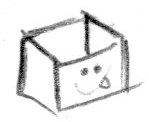
\includegraphics[scale=1]{devices/pint}
                    \vspace{-20pt}
                \end{wrapfigure}

                Containers for regular ice cream. Depending on the level, the cups may be bigger in order to be capable of containing more scoops of ice cream obtained from multiple runs through dosers.
            \end{minipage}

        \subsubsection{Popsicle molds}
            \begin{minipage}[t][3em][t]{\textwidth}
                \begin{wrapfigure}{l}{0.1\textwidth}
                    \vspace{-15pt}
                    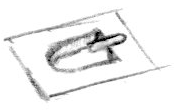
\includegraphics[scale=1]{devices/popsicle_molds}
                    \vspace{-25pt}
                \end{wrapfigure}

                Containers (with wooden sticks) for Popsicles. Differently than the ice cream cups, the Popsicle molds have a standard size.
            \end{minipage}

        \subsubsection{Banana plates}
            \begin{minipage}[t][2em][t]{\textwidth}
                \begin{wrapfigure}{l}{0.1\textwidth}
                    \vspace{-20pt}
                    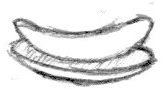
\includegraphics[scale=1]{devices/banana_plate}
                    \vspace{-25pt}
                \end{wrapfigure}

                Special containers with a banana divided in half, used for preparing banana-splits.
            \end{minipage}

    \subsubsection{Production Devices}
        The production devices are responsible for bringing the production line to life!
        In other words, these are the devices that will dispense the containers, fill them with ice cream and cover them with toppings and candies.

		\subsubsection{Container Dispensers}
            \begin{minipage}[t][6em][t]{\textwidth}
                \begin{wrapfigure}[5]{l}{0.16\textwidth}
                    \vspace{-20pt}
                    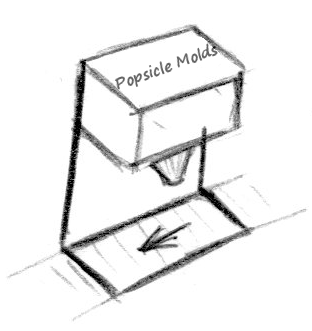
\includegraphics[scale=1]{devices/container_dispenser}
                    \vspace{-20pt}
                \end{wrapfigure}

                These devices dispense containers for ice cream of a configured type and quantity. The player places one of these devices in the conveyor belt and configures it for which type of container is required. Action buttons are used to define the number of containers to be dispensed, ranging from 1 to 10. After the production line is started, the containers will be dispensed in regular intervals (each two conveyor cycles) until that number is reached.
            \end{minipage}			

        \subsubsection{Ice Cream Dosers}
            \begin{minipage}[t][7em][t]{\textwidth}
                \begin{wrapfigure}[5]{l}{0.16\textwidth}
                    \vspace{-20pt}
                    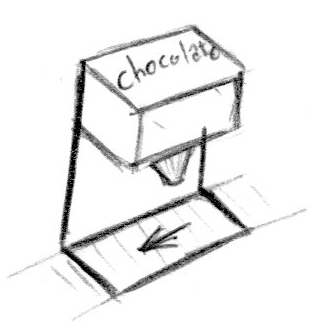
\includegraphics[scale=1]{devices/ice_cream_doser}
                    \vspace{-20pt}
                \end{wrapfigure}

                These devices dispense one single scoop of ice cream in the configured flavor into a container when one is located underneath it. They work with all types of containers in the same way, be it cups, Popsicle molds and banana plates. A doser can dispense ice cream in only one flavor, selected by the player before the production line is started. The flavor is selected by touching (or clicking) the device in a rotation manner (each touch selects the next flavor in a circular list).
                \\
                The existing ice cream flavors are: milk cream, strawberry, chocolate, mint and vanilla.
            \end{minipage}

        \subsubsection{Topping Dosers}
            \begin{minipage}[t][6em][t]{\textwidth}
                \begin{wrapfigure}[5]{l}{0.16\textwidth}
                    \vspace{-20pt}
                    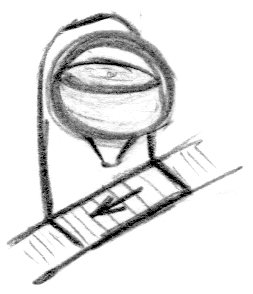
\includegraphics[scale=1]{devices/topping_doser}
                    \vspace{-10pt}
                \end{wrapfigure}

                These devices work in the same way of the ice cream dosers, but dispensing topping flavors instead. They dispense only one measure of topping when a container is underneath it. The topping flavor dispensed is also selected by touching the device, before the production line is started.
                \\
                The existing topping flavors are: hot fudge (chocolate), hot fudge (caramel), chocolate chips, walnuts and sweet crumbs.
            \end{minipage}

        \subsubsection{Candy Dispensers}
            \begin{minipage}[t][6em][t]{\textwidth}
                \begin{wrapfigure}{l}{0.2\textwidth}
                    \vspace{-20pt}
                    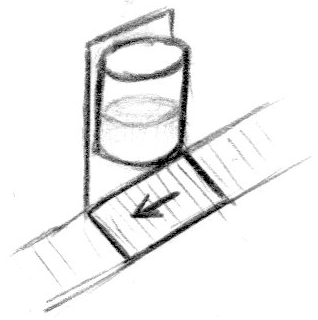
\includegraphics[scale=1]{devices/special_topping_doser}
                    \vspace{-20pt}
                \end{wrapfigure}

                Similar to topping dosers, these devices dispense candies like marshmallows, Oreo crackers and waffle tubes. Only one candy is dispensed by each pass of a container underneath the device.
            \end{minipage}

    \subsection{Control Devices}
    	The production devices have their limitations, mainly they are only able to dispense one scoop, measure or candy per time a cup pass underneath them. But the customers sometimes require two scoops of chocolate, an extra waffle tube or two measures of walnuts in their ice creams! Also, the number of devices available in each level is restricted. So, in order to cope with that, it is sometimes necessary to conduct the ice creams pots, Popsicle molds or banana plates under the production devices more than once. This is a big part of the challenges in \gamename.
    	
    	In order to control the path performed by the fixed layout of conveyors, the player uses control devices.

        \subsubsection{Switchers}
            \begin{minipage}[t][7em][t]{\textwidth}
                \begin{wrapfigure}{l}{0.2\textwidth}
                    \vspace{-20pt}
                    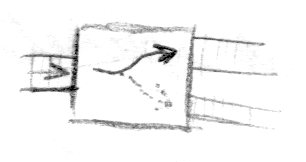
\includegraphics[scale=1]{devices/switcher}
                    \vspace{-15pt}
                \end{wrapfigure}

                Switchers are the simplest path control devices. They need to be placed in existing forks on the conveyor belt (where a track leads to two other possible tracks). They conduct a passing product to a given track and are toggled (changed) after the product passes, then conducting the next product to the other track. For instance, the first product passing is conducted to track A, when the switcher is then toggled so the second product passing is conducted to track B. The switcher is toggled again, so the third product passing will be conducted again to track A. And so on. The initial direction of the switcher (that is, before the production line is started), is defined by the player by touching the switcher action button.
            \end{minipage}

        \subsubsection{Weighing Scales}
            \begin{minipage}[t][8em][t]{\textwidth}
                \begin{wrapfigure}{l}{0.2\textwidth}
                    \vspace{-20pt}
                    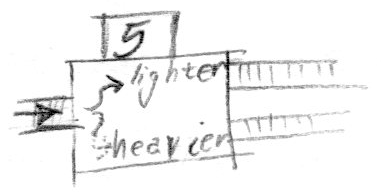
\includegraphics[scale=1]{devices/scale}
                    \vspace{-20pt}
                \end{wrapfigure}

                The weighing scales are also switchers, but that change state (that is, the track to which they conduct products) based on the measured weighted of a product. Once the product arrives at a scale device, it is weighted. If the product's weight is greater than the device configured value, the product will be conducted to the ``heavier'' track and otherwise to the ``lighter'' track.
                \\
                For simplicity, all scoops of ice cream, measures of toppings and unities of candy weight one (1). The device configured weight is also set up by touching (or clicking) on up and down action buttons connected to it. The possible values are in integer numbers, ranging from 1 to 10.
            \end{minipage}
            
		\subsubsection{Counting Scales}
            \begin{minipage}[t][8em][t]{\textwidth}
                \begin{wrapfigure}{l}{0.2\textwidth}
                    \vspace{-20pt}
                    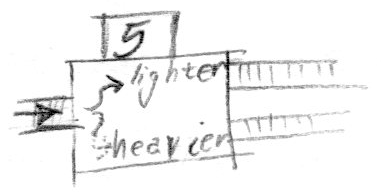
\includegraphics[scale=1]{devices/scale}
                    \vspace{-20pt}
                \end{wrapfigure}

                Similar to the weighing scales, but instead of weighting a product this type of switcher counts the number of products that have passed so far through it. Once the configured maximum number of products passed, it changes to the other path allowing one more product to pass. It then resets the counter back to zero. The maximum counter value is defined by the user by touching (or clicking) the action buttons, ranging from 1 to 10.
            \end{minipage}            

        \subsubsection{Tasters}
            \begin{minipage}[t][5em][t]{\textwidth}
                \begin{wrapfigure}{l}{0.24\textwidth}
                    \vspace{-20pt}
                    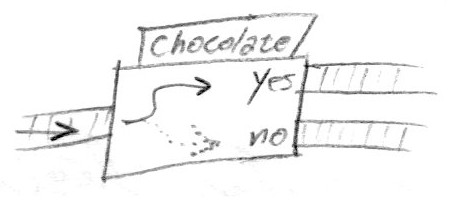
\includegraphics[scale=1]{devices/taster}
                    \vspace{-20pt}
                \end{wrapfigure}

                Tasters are also switchers, but they check whether the ice cream flavor is the same of a specified one. If the flavor is the same as the one configured, the product goes to the ``yes'' track and otherwise to the ``no'' track. The pot is also conducted to the ``no'' track if it is empty. The player can set the taster verification flavor by also clicking the device, in a circular fashion.
            \end{minipage}

\section{Game Mechanics}

	\subsection{Interaction}
		The game is played by touch or mouse cursor. In each level, the game screen will present a fixed layout of conveyors forming the production line. Each straight segment will have an arrow indicating the direction in which the conveyors are running. In a separated area, the player will be presented with the devices and their quantities available for using in the building of her factory.
		
		The player selects or de-selects a device by touching or clicking it. A selected device is placed in game by touching or clicking again over a conveyor in the production line. Devices already in place can be moved by the same process: a selected device can be moved to another location by touching or clicking in the new location, or removed from the game back in the devices area by touching or clicking in there.
		
		Each device has one or two action buttons, allowing the player to set up their configurations by simply touching or clicking the buttons. Container dispensers, for instance, have one button that allows toggling among the existing options for ice cream containers. Counting and weighing switchers, for instance, have two buttons: one for increasing and another for decreasing the device configuration value. Regular switches also have a button, but for defining the default direction. Same for Tasters, which have a button for toggling among the flavors to be tested.
		
		The main screen has two other buttons: one for starting the production line, and another for reseting all the devices (put them back to the device area). Another button gives access back to the main menu. Once the production line is started, the conveyors will start to run, and all devices positioned will work when appropriated (container dispensers will work in a fixed rate, and dosers and control devices will work when an ice cream container is traveling through them).
		
	\subsubsection{Rewards}
		One first playing the game, only the first level is unlocked. A player has to succeed in solving the current puzzle to have access to the next level. Also, new truck drivers will be unlocked as the player progress in the game. Their profile sheets will be collected and displayed in a proper section, accessible from the game's main menu.
		
		The initial levels will be much easier to solve, but more difficult levels composed of more complex paths will allow different solutions, sometimes involving the use of less devices. In that case, the player will be granted with one to three starts depending on the solution achieved.
		
	\subsubsection{Example Levels}
		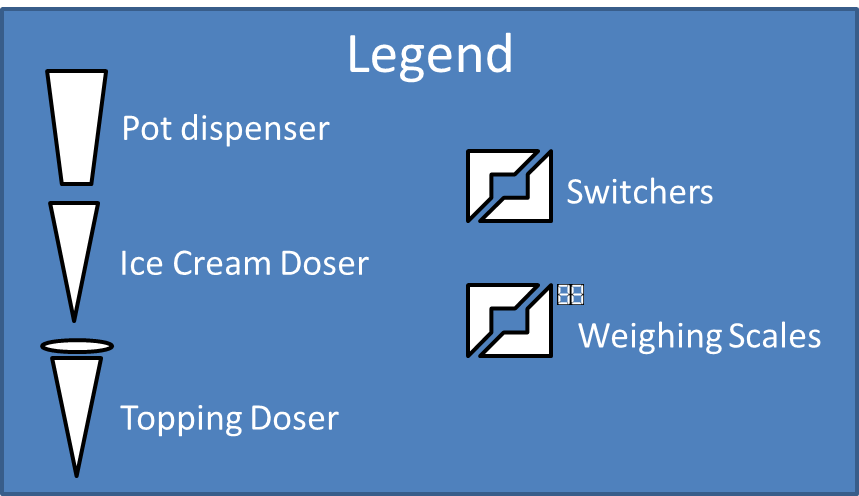
\includegraphics[width=\textwidth]{levels/legend}
		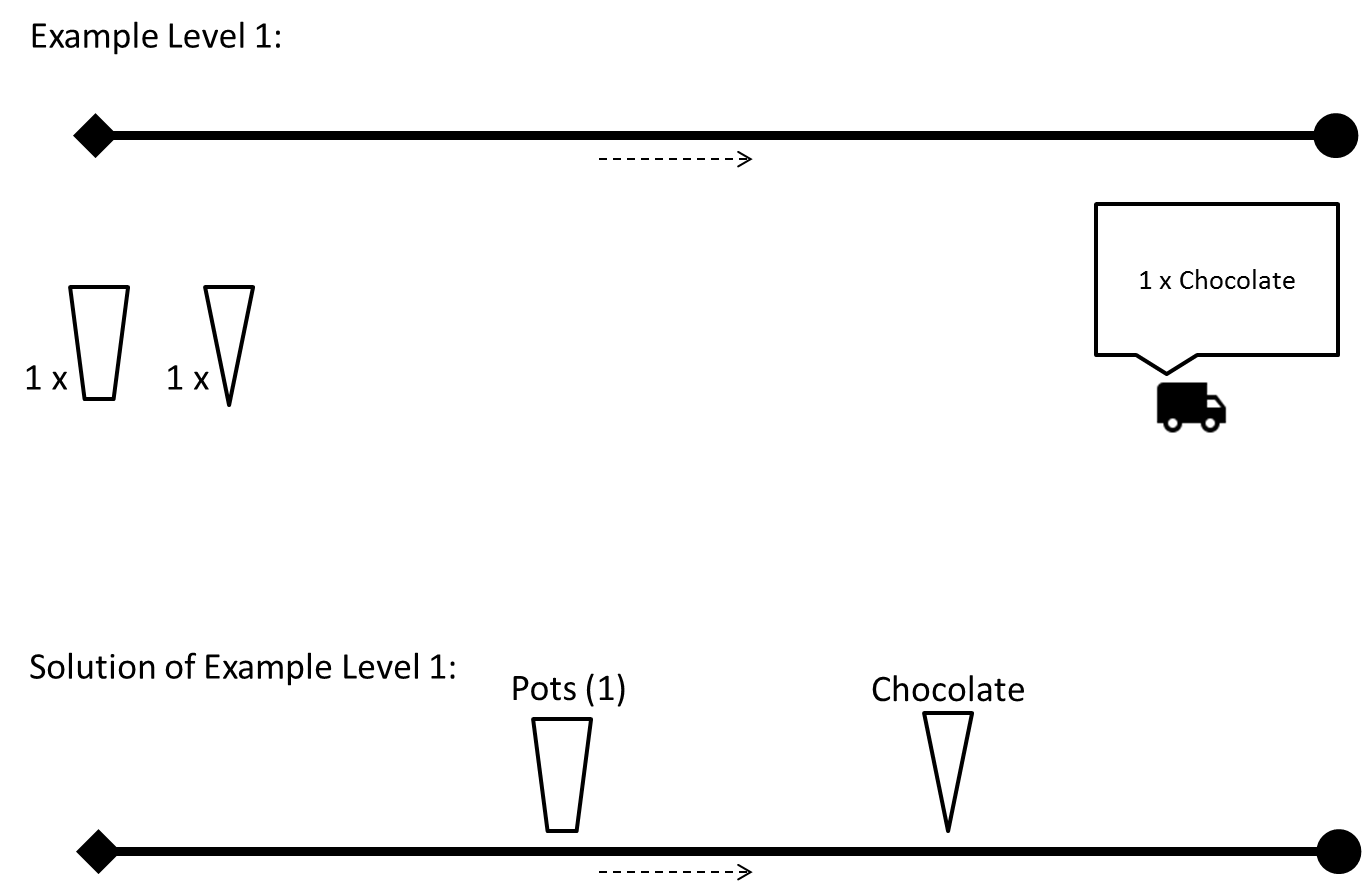
\includegraphics[width=\textwidth]{levels/01}
		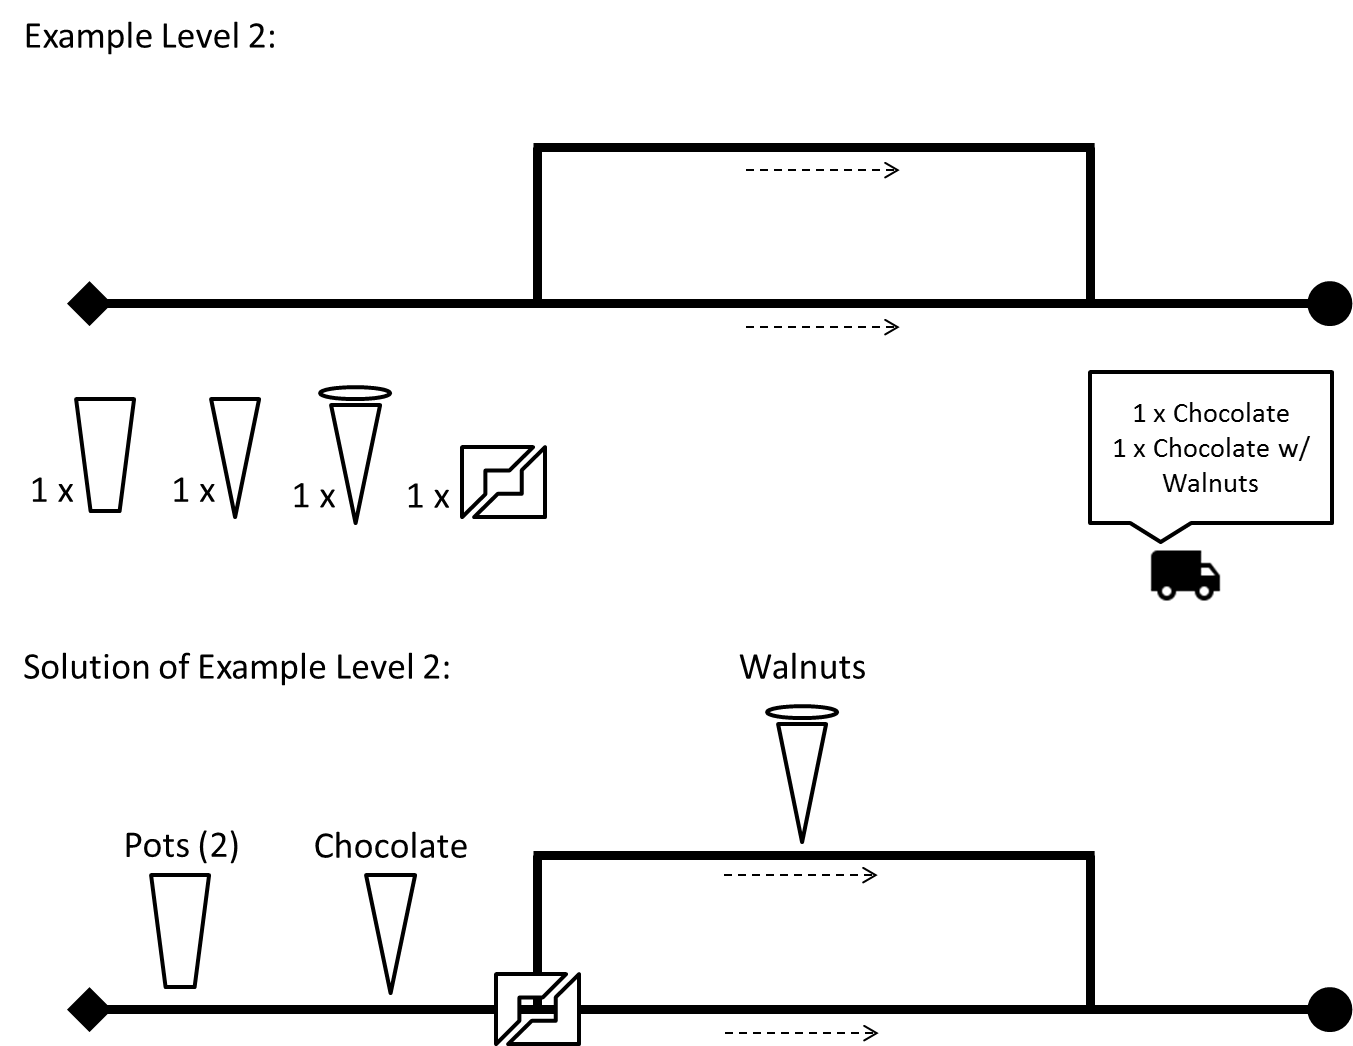
\includegraphics[width=\textwidth]{levels/02}
		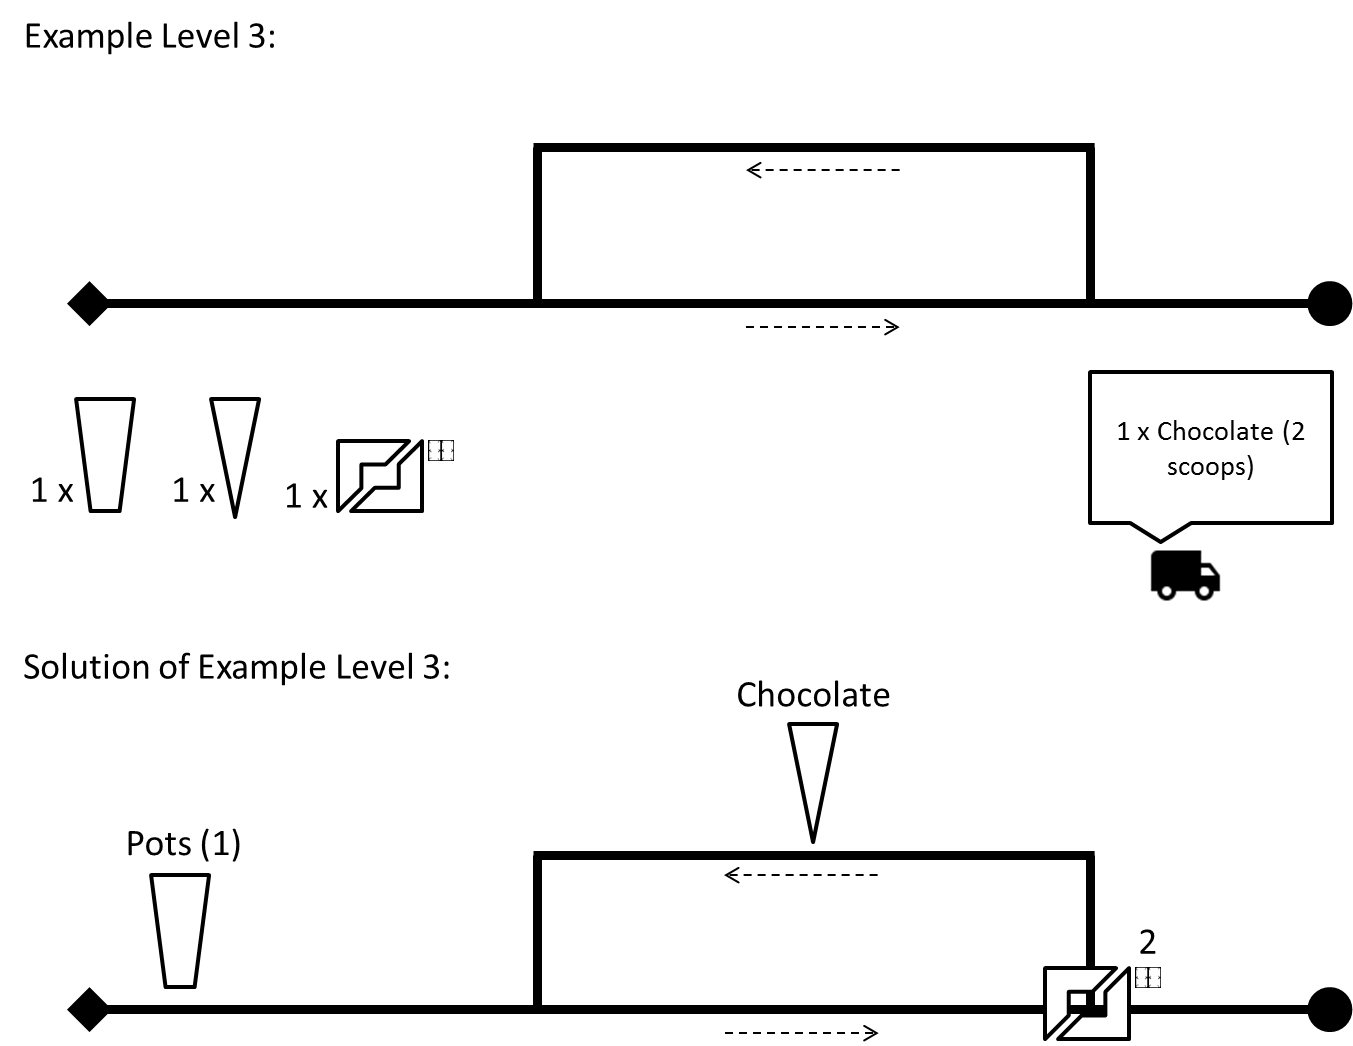
\includegraphics[width=\textwidth]{levels/03}
		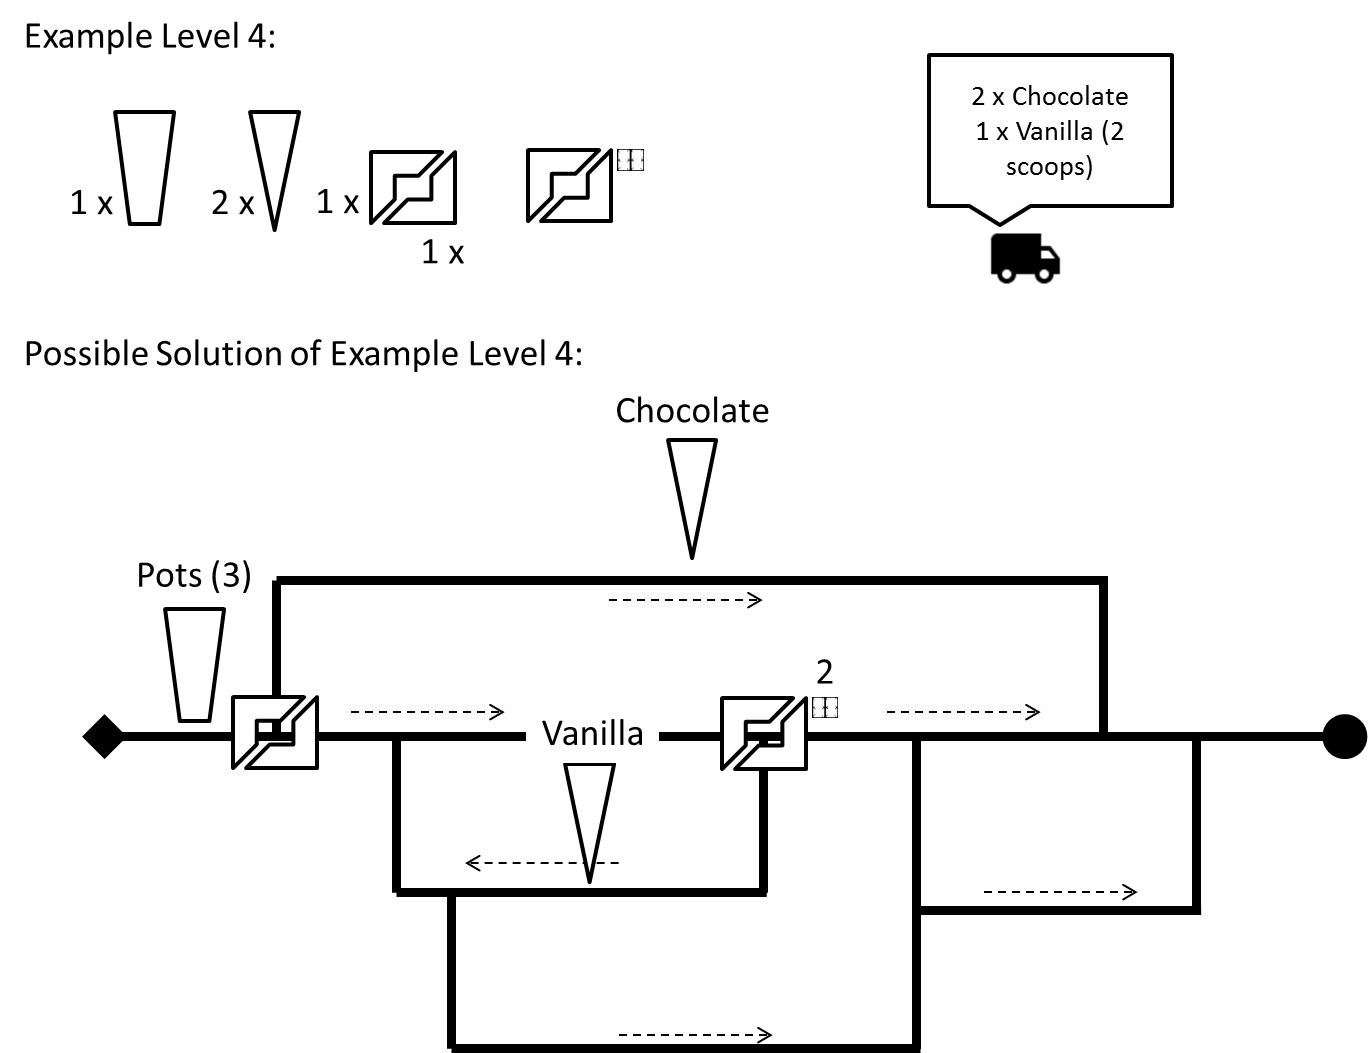
\includegraphics[width=\textwidth]{levels/04}

\section{Concept art}
    Here there are a few images to show the visual identity planned for \gamename.

    \centering
    \begin{multicols}{2}
       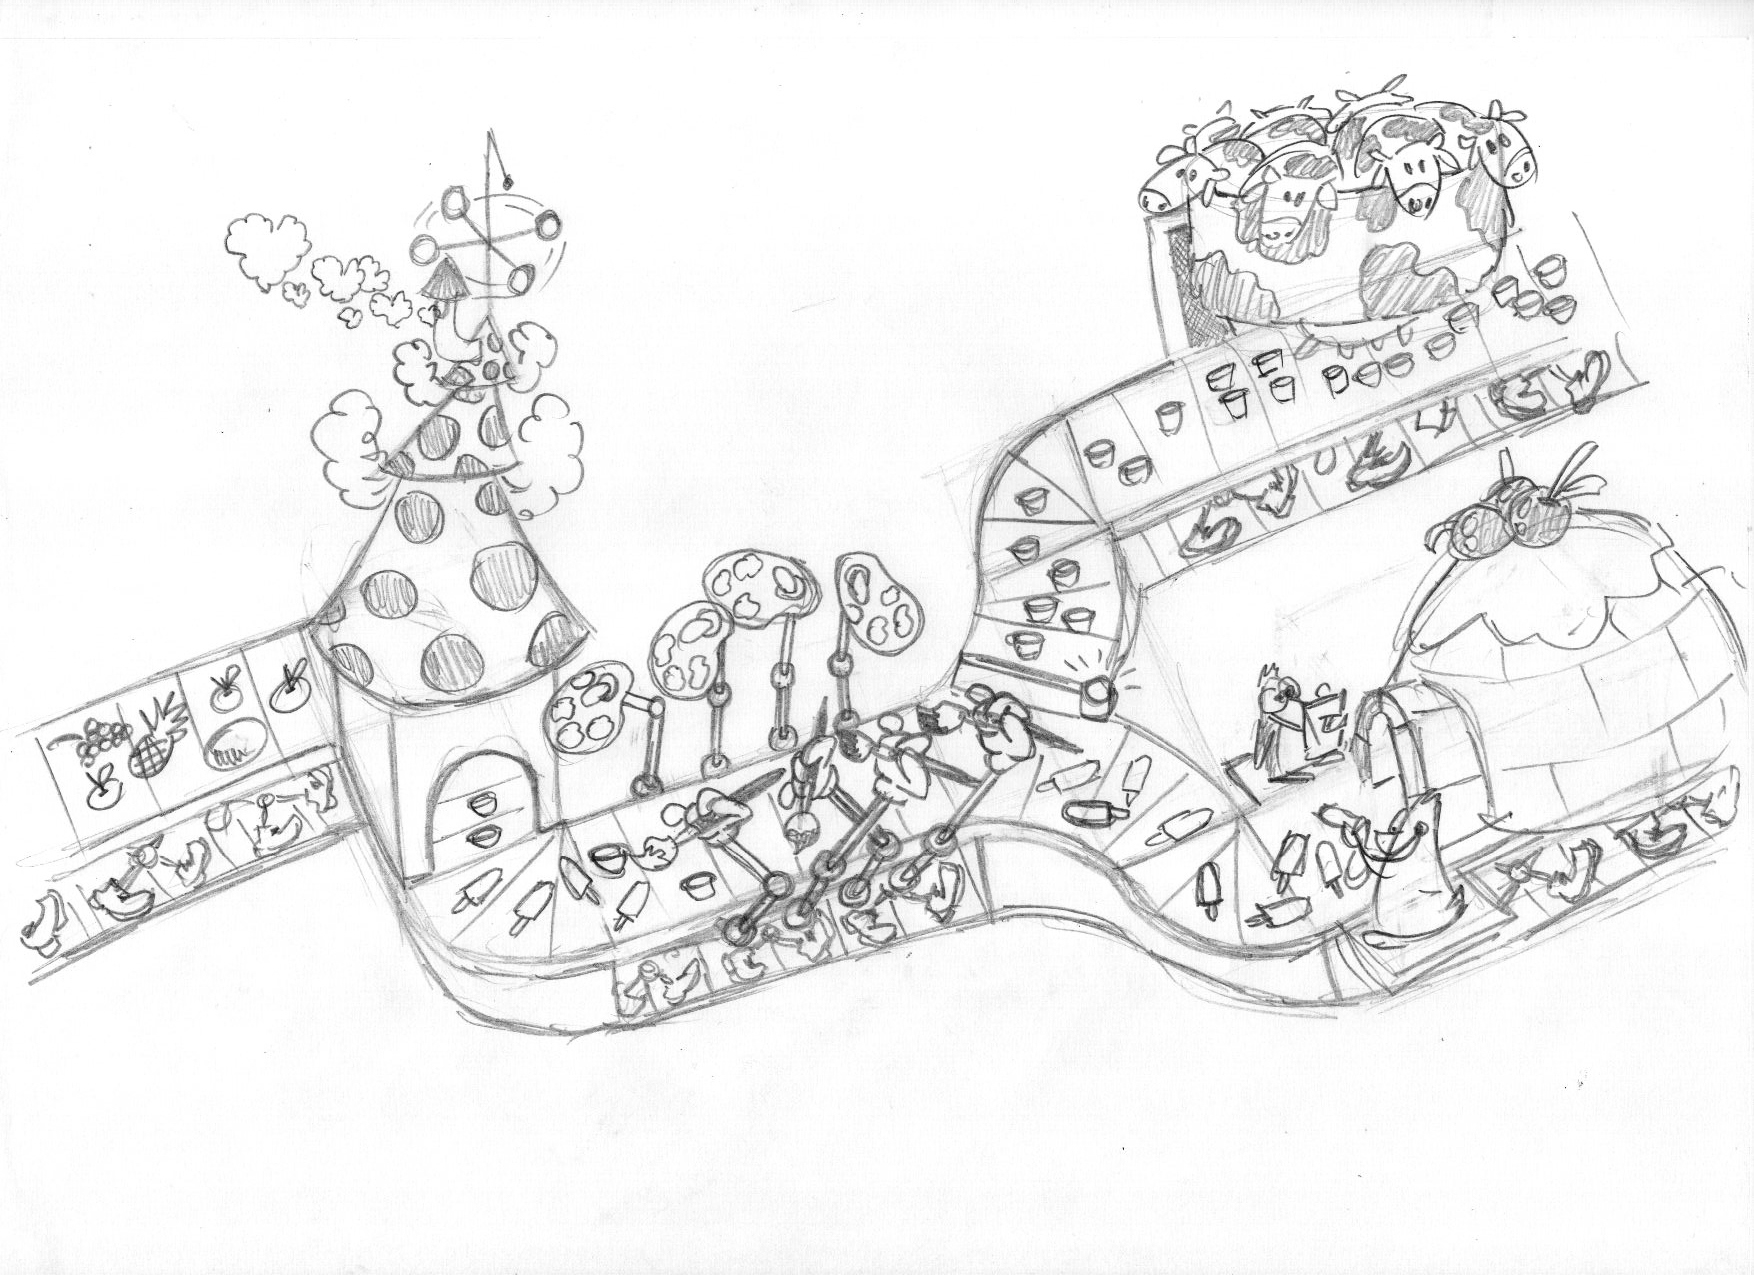
\includegraphics[width=0.49\textwidth]{references/01}

       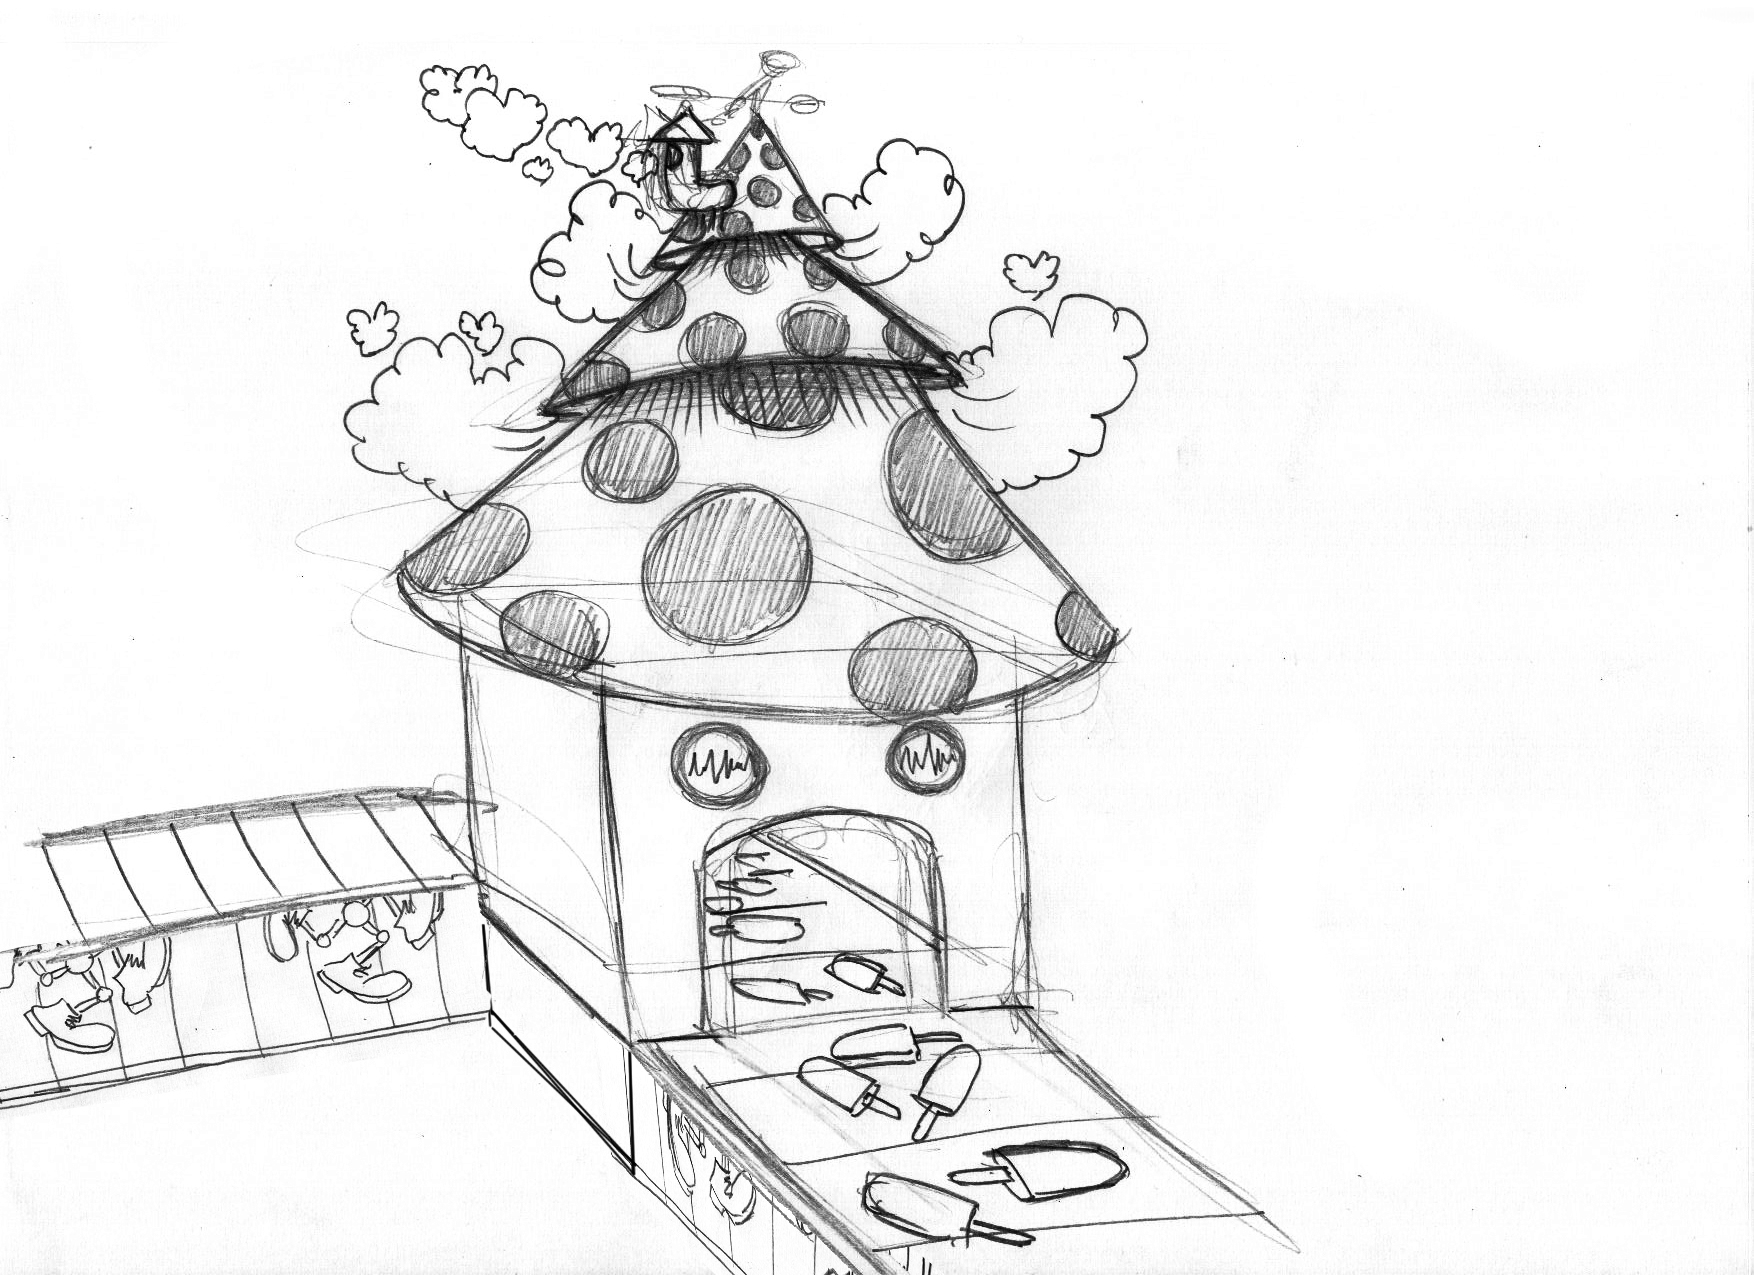
\includegraphics[width=0.49\textwidth]{references/02}
    \end{multicols}
    
    \begin{multicols}{2}
       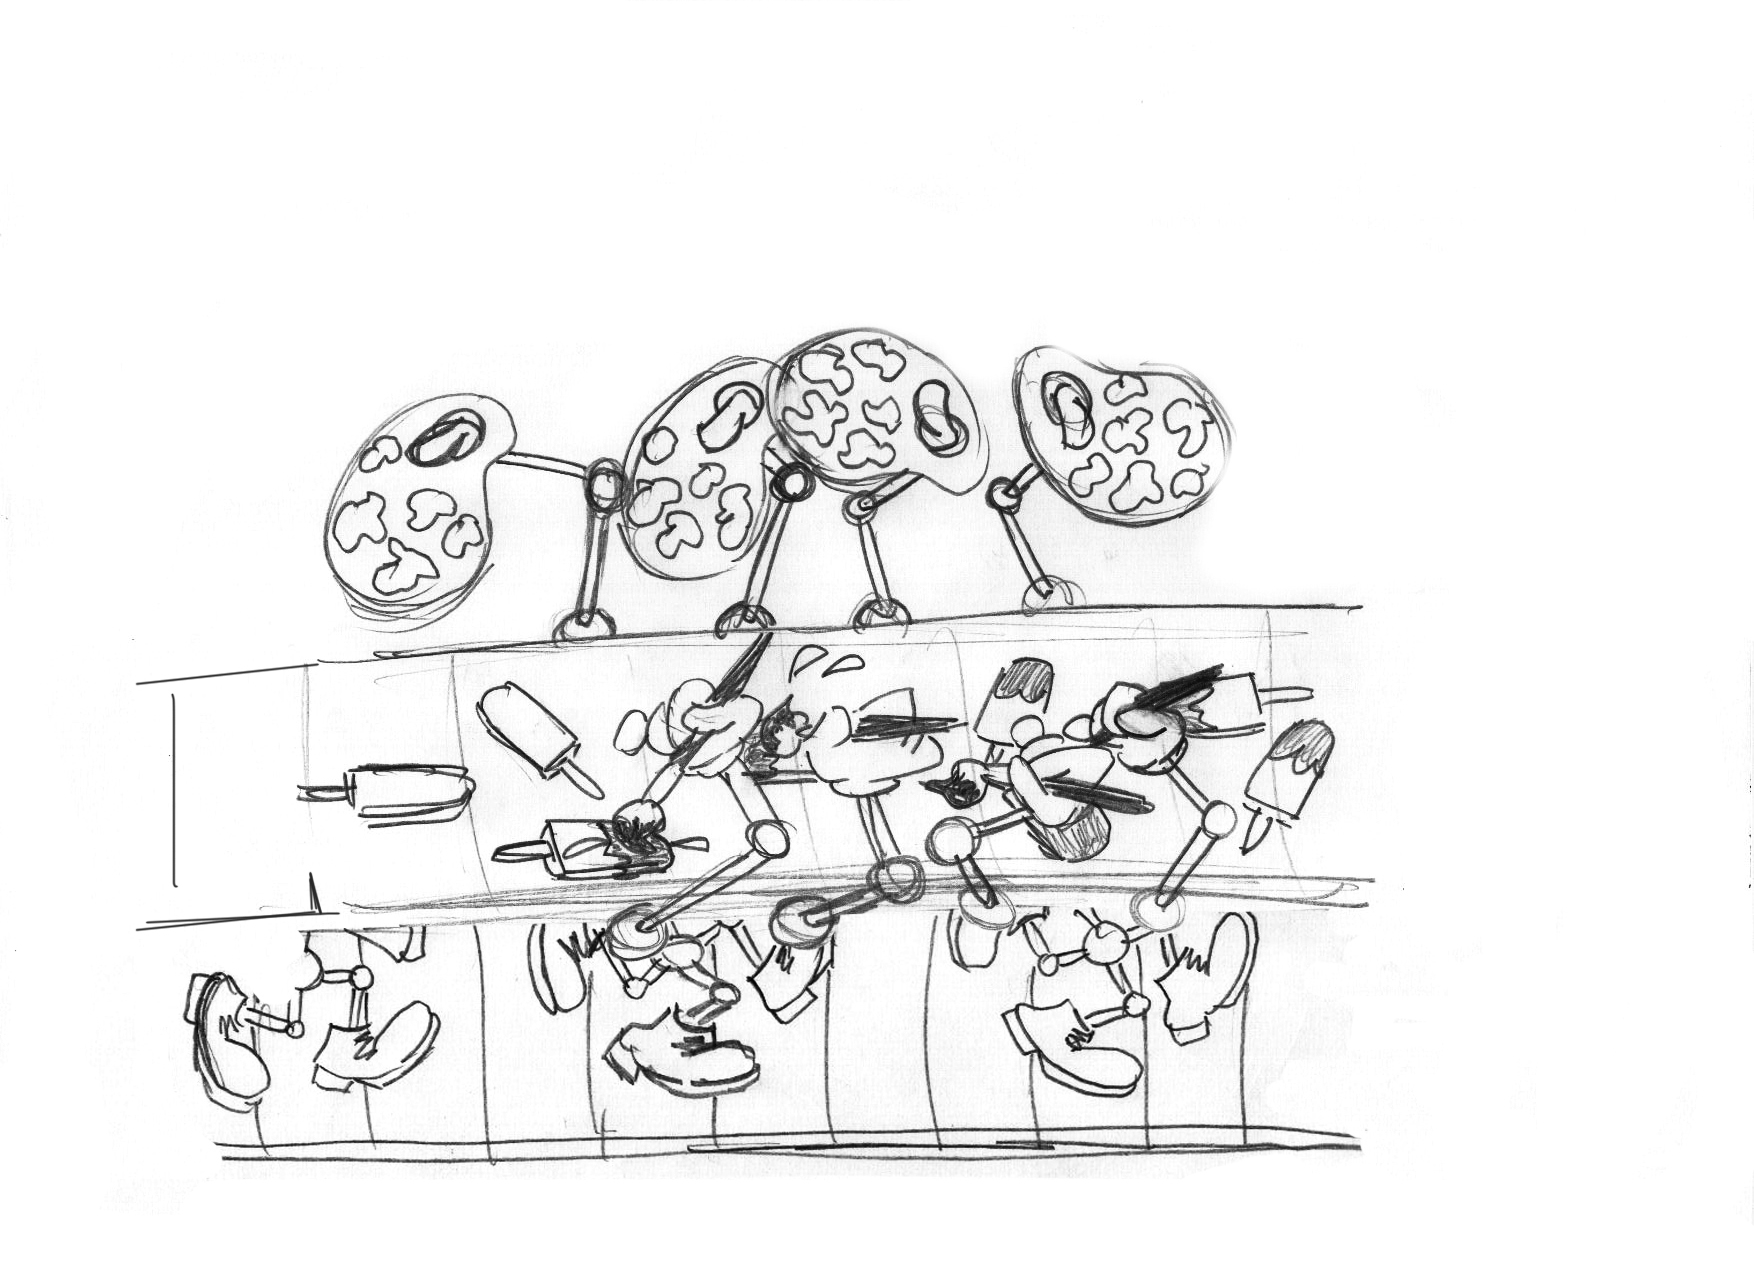
\includegraphics[width=0.49\textwidth]{references/03}

       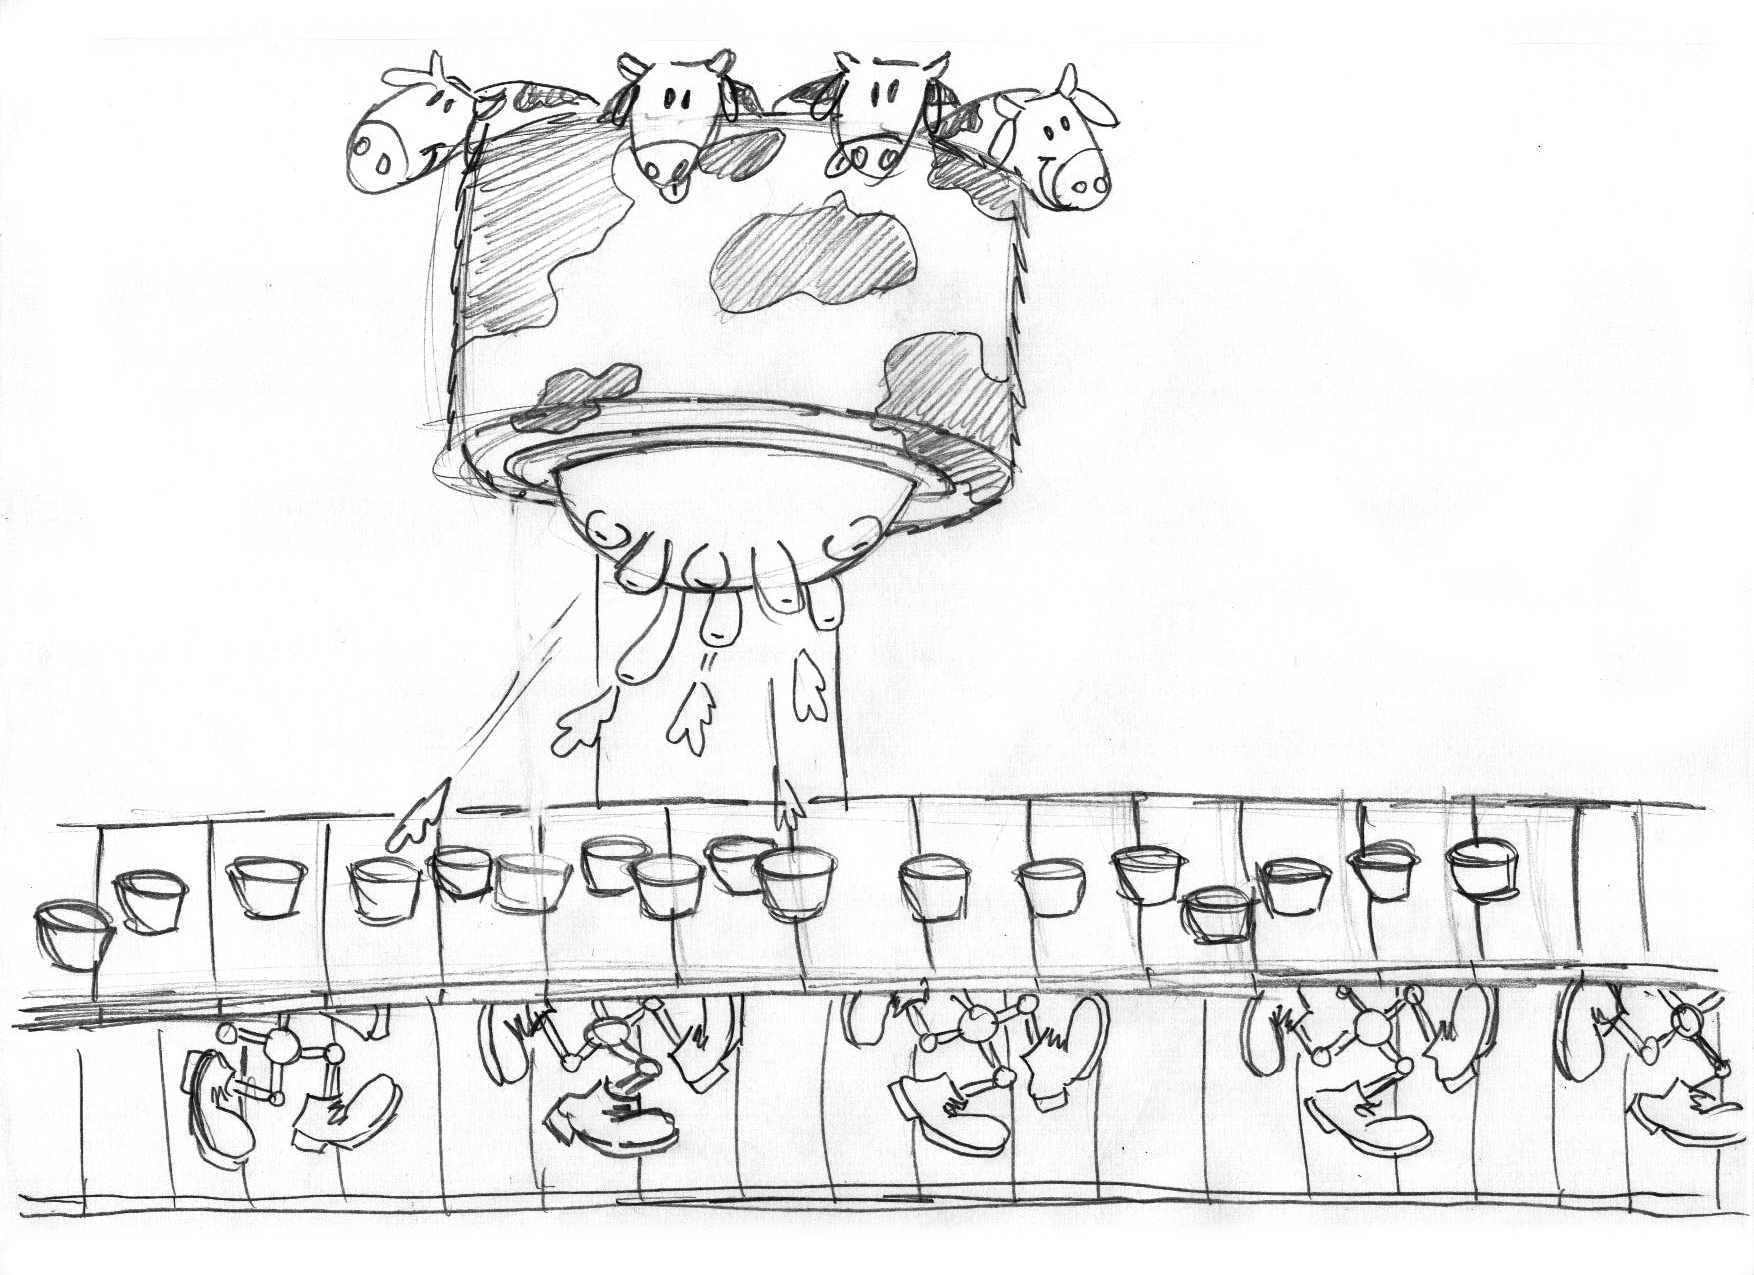
\includegraphics[width=0.49\textwidth]{references/04}
    \end{multicols}
    
    \begin{multicols}{2}
       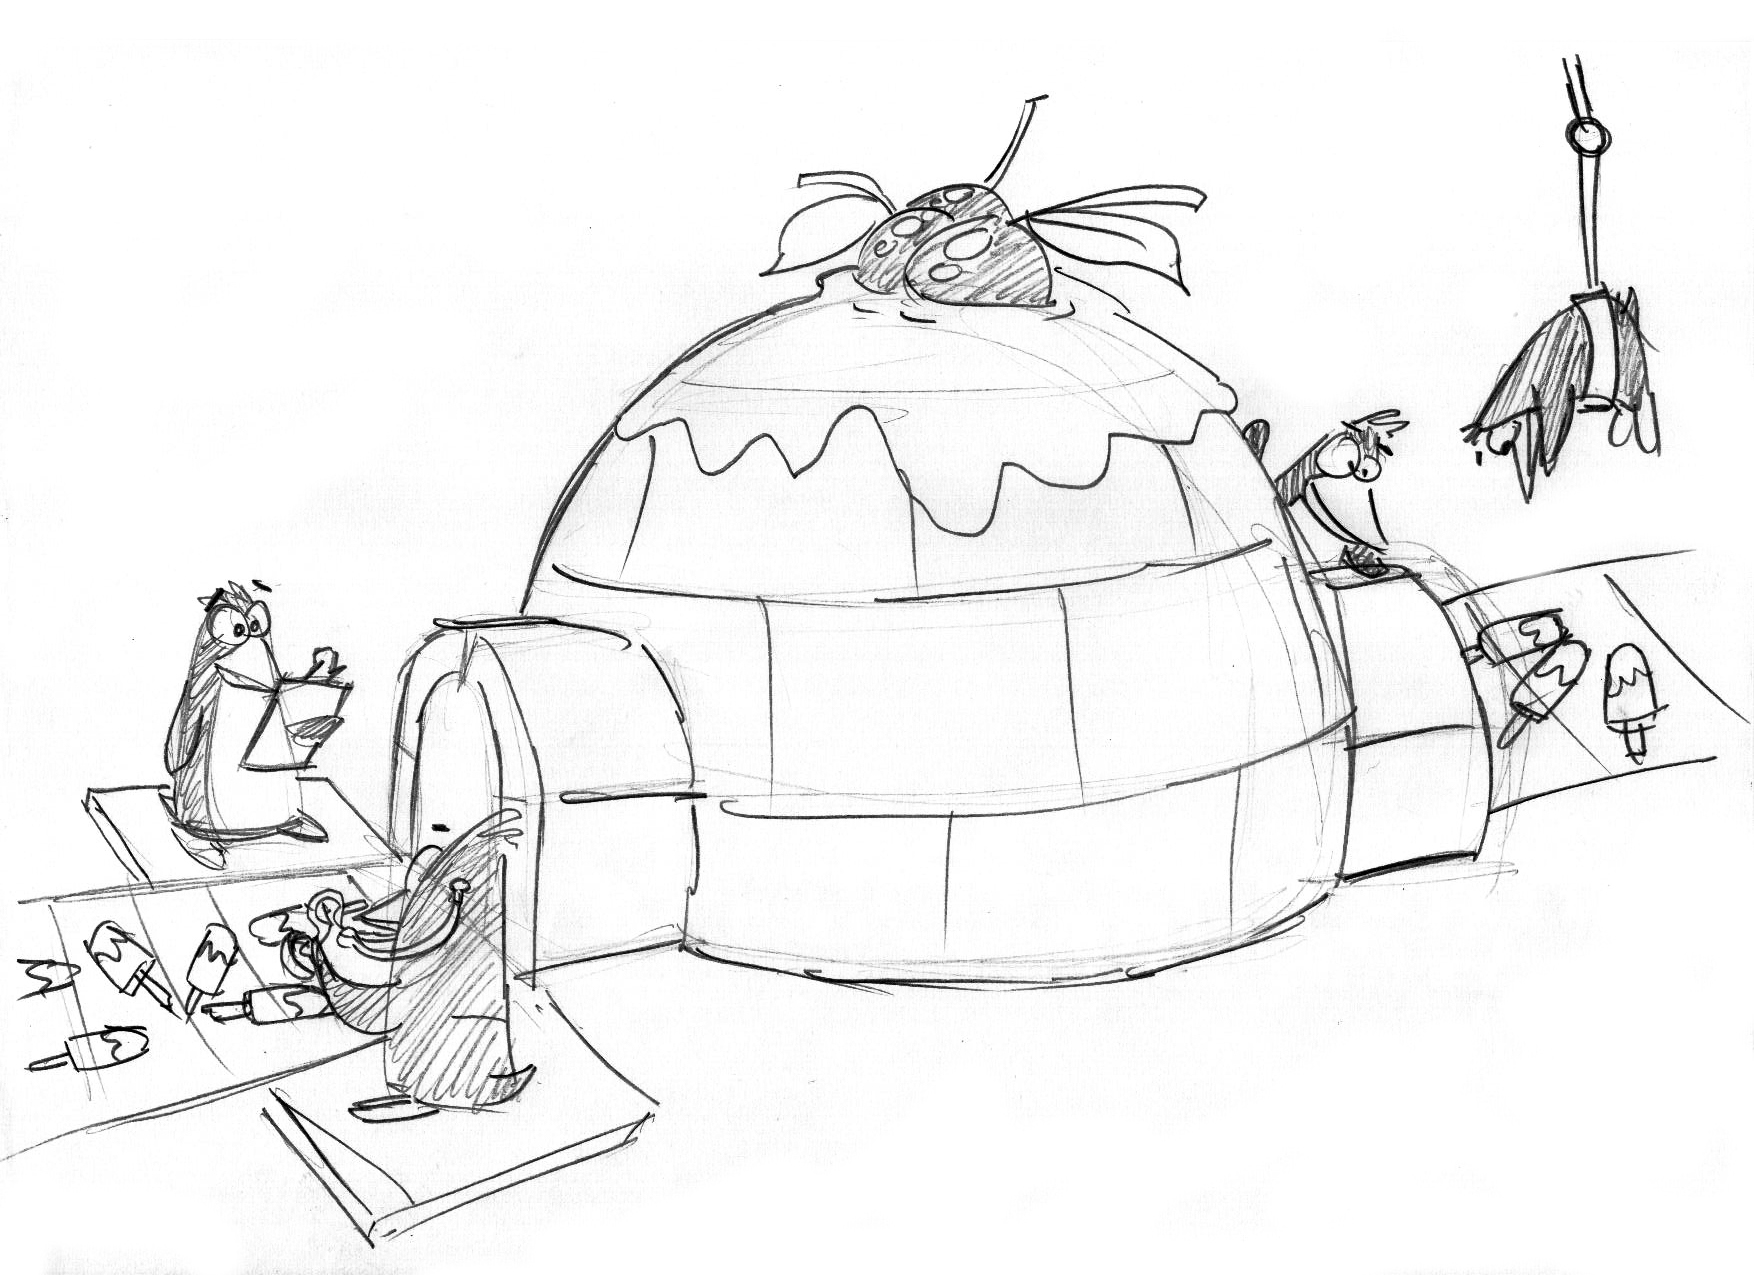
\includegraphics[width=0.49\textwidth]{references/05}

       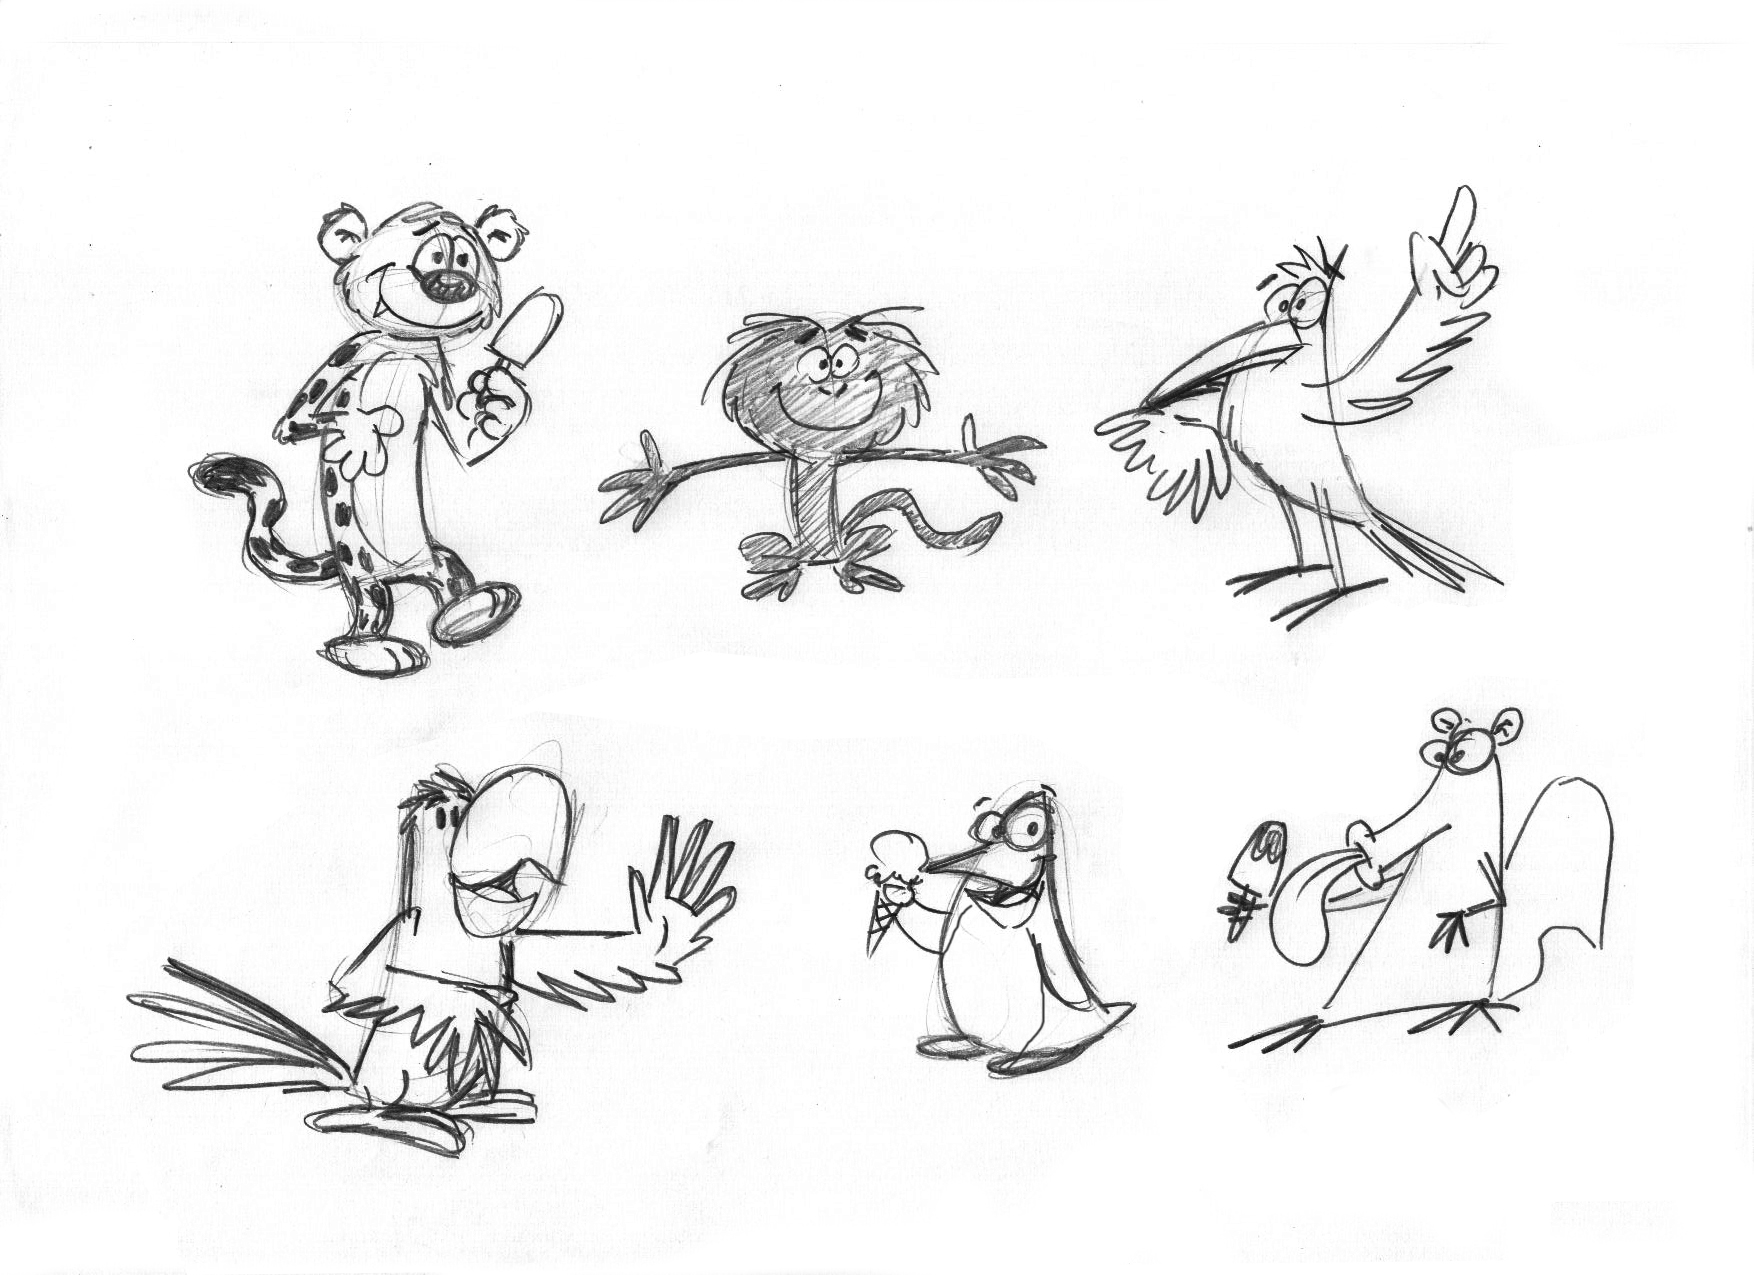
\includegraphics[width=0.49\textwidth]{references/06}
    \end{multicols}    

\section{Similar games}
    In this section we can see some factory games which have the same conveyor
    concept present in \gamename.

    \begin{multicols}{2}
        \subsection{Cake Factory - Barbie Games}
            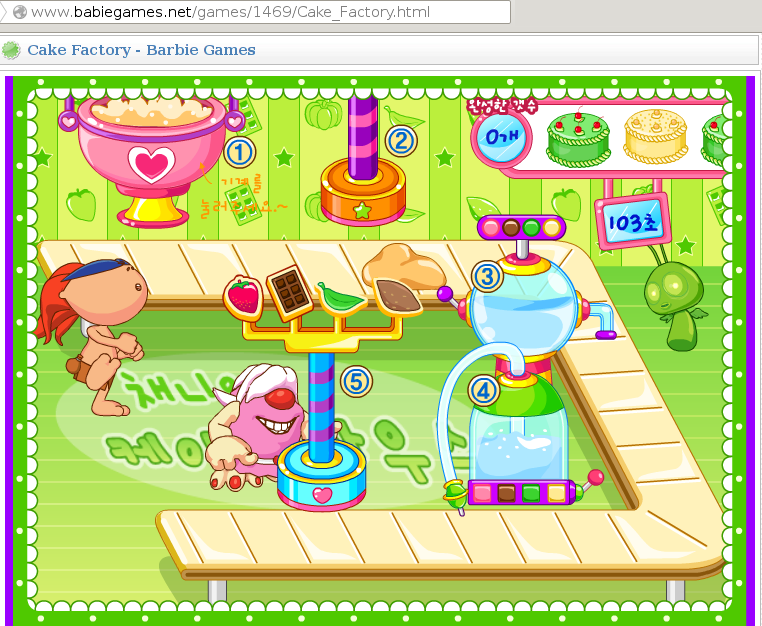
\includegraphics[width=0.49\textwidth]{similar_games/CakeFactory}

        \subsection{Toy Factory Fun}
            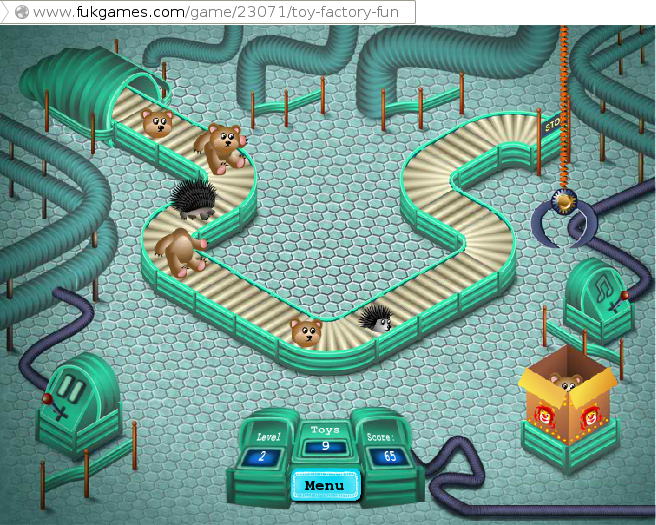
\includegraphics[width=0.49\textwidth]{similar_games/ToyFactoryFun}
    \end{multicols}

    \begin{multicols}{2}
        \subsection{Jewel Factory}
            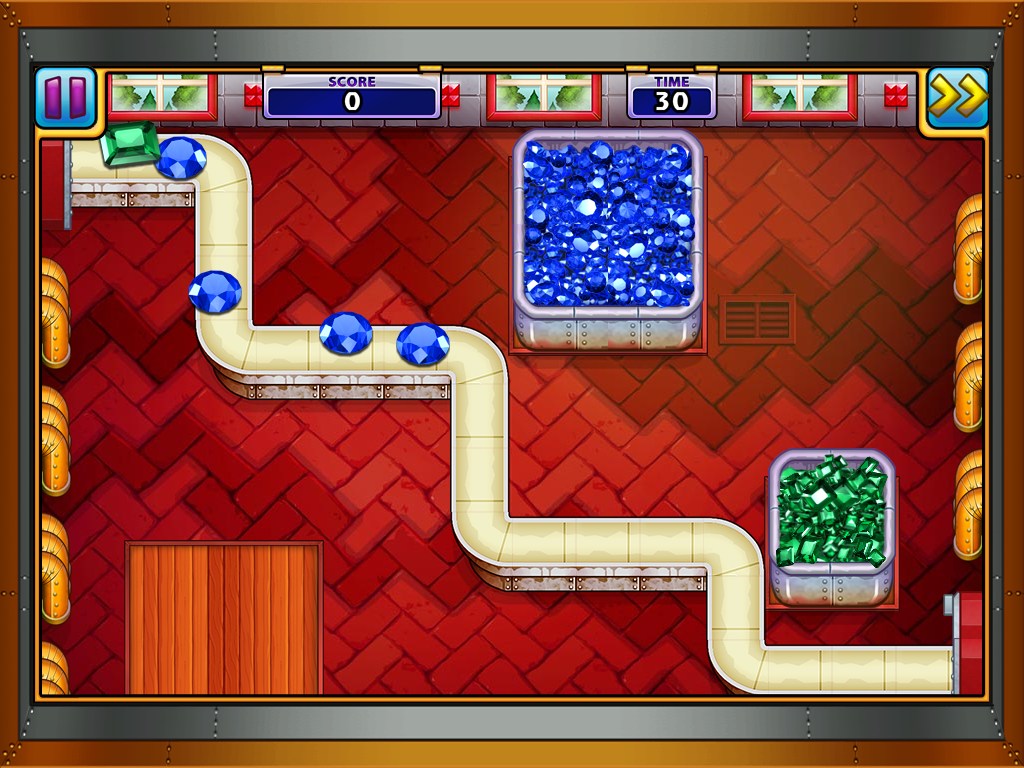
\includegraphics[width=0.49\textwidth]{similar_games/JewelFactory}

        \subsection{Production Panic}
            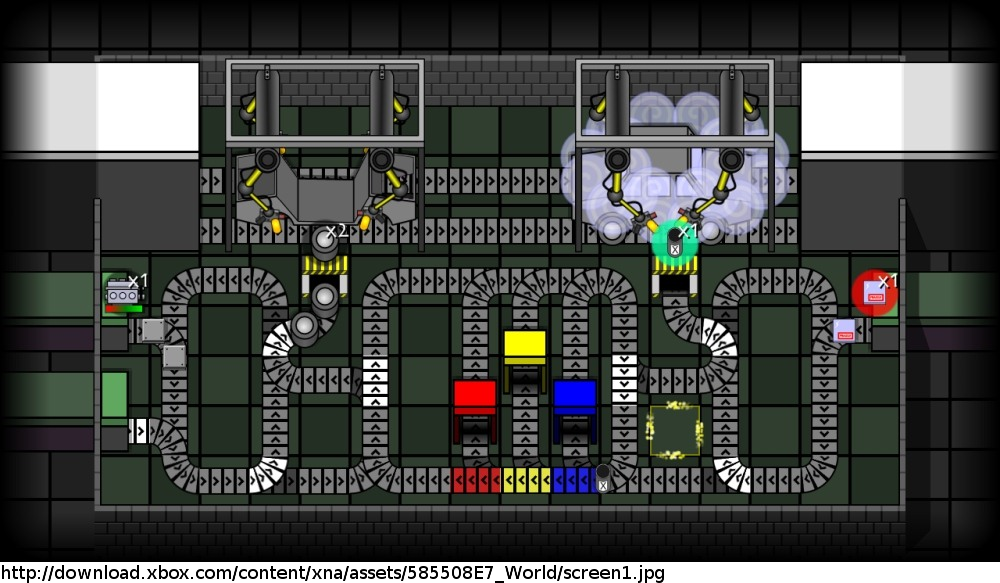
\includegraphics[width=0.49\textwidth]{similar_games/ProductionPanic}
    \end{multicols}

    \begin{multicols}{2}
        \subsection{Candy Factory - LeeGT}
            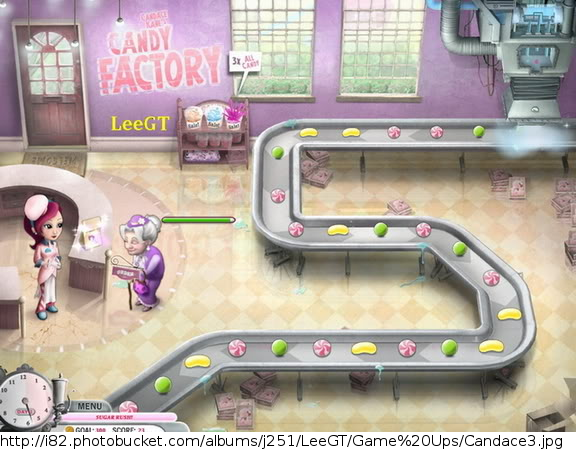
\includegraphics[width=0.49\textwidth]{similar_games/CandyFactoryLeeGT}

        \subsection{Teddy Factory}
            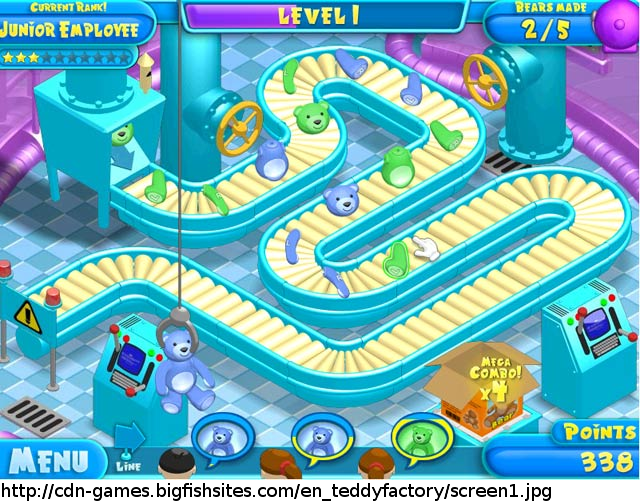
\includegraphics[width=0.49\textwidth]{similar_games/TeddyFactory}
    \end{multicols}

    \begin{multicols}{2}
        \subsection{Robot Factory}
            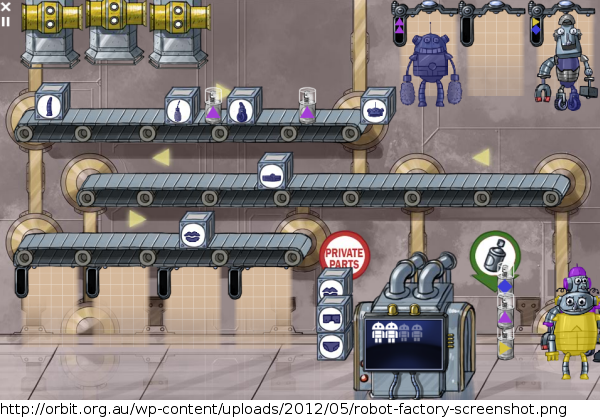
\includegraphics[width=0.49\textwidth]{similar_games/RobotFactory}

        \subsection{Space Chem}
            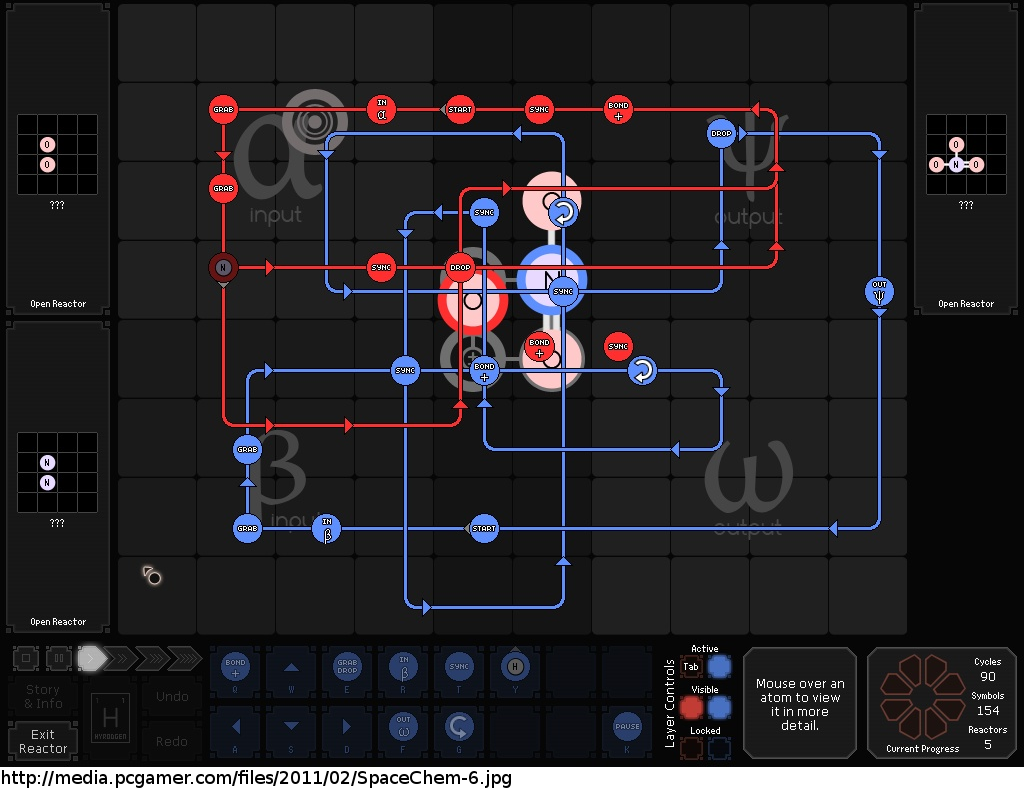
\includegraphics[width=0.49\textwidth]{similar_games/SpaceChem}
    \end{multicols}

    \begin{multicols}{2}
        \subsection{Candy Conveyors}
            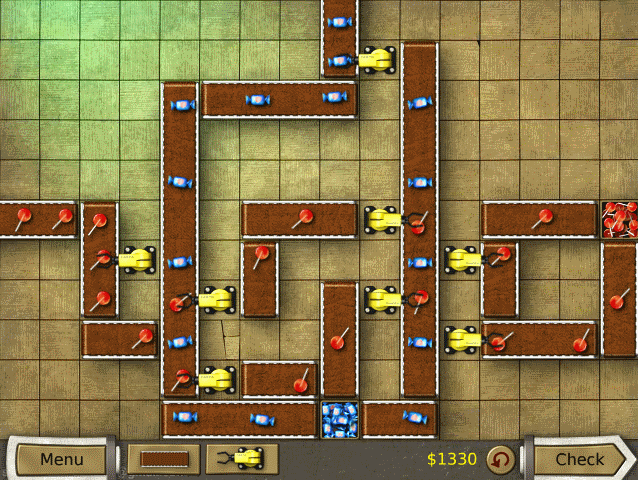
\includegraphics[width=0.49\textwidth]{similar_games/CandyConveyors}

        \subsection{The Cake Factory}
            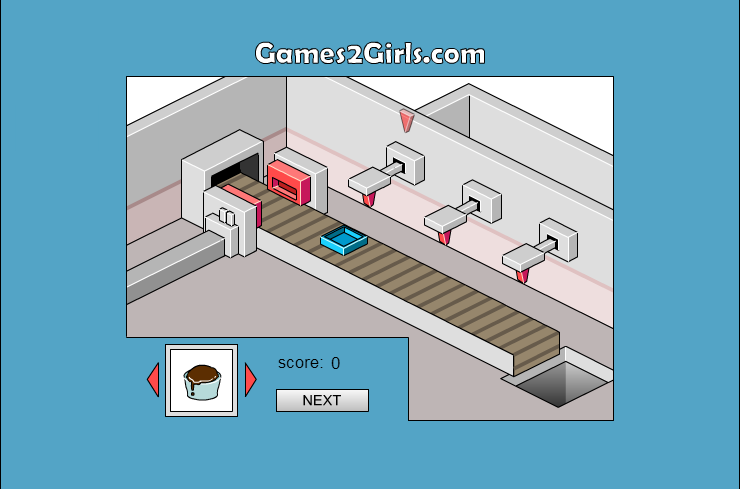
\includegraphics[width=0.49\textwidth]{similar_games/TheCakeFactory}
    \end{multicols}

\section{Game name alternatives}
    \begin{itemize}
        \item Smart Factory
        \item Smart Cream
        \item Smart Ice Cream Factory
        \item Smart Split
        \item Ice Cream Factory
        \item Favorite Flavors (\textit{Sorvetes Sortidos})
    \end{itemize}

\end{document}
